\documentclass{beamer}

\usepackage[utf8]{inputenc}
\usepackage[T1]{fontenc}
\usepackage[ngerman]{babel}
\usepackage{graphicx} % Bilder
\usepackage{wrapfig} % Umflussbilder
\usepackage{multicol} % Multiple columns
\usepackage{minted} % Haskell source code
\usepackage{framed} % Frames around source code
\usepackage[framemethod=tikz]{mdframed} % Frames
\usepackage{verbatim} % \begin{comment}...\end{comment}
\usepackage{etoolbox} % manipulate minted
\AtBeginEnvironment{minted}{\fontsize{10}{10}\selectfont}
\AfterEndEnvironment{minted}{}

\mdfdefinestyle{fancy}{
  roundcorner=5pt,
  linewidth=4pt,
  linecolor=red!80,
  backgroundcolor=red!20
}
\newmdenv[style=fancy]{important}

% redifine \em for \emph to use bold instead of italics
\makeatletter
\DeclareRobustCommand{\em}{%
  \@nomath\em \if b\expandafter\@car\f@series\@nil
  \normalfont \else \bfseries \fi}
\makeatother

% Stuff for Beamer
\beamertemplatenavigationsymbolsempty
\usetheme{Warsaw}

\title{Fortgeschrittene Funktionale Programmierung in Haskell}

\begin{document}
  
%----------------------------------------------------------------------------------------  

  \begin{frame}
  \begin{center}
    \huge\textbf{Fortgeschrittene Funktionale Programmierung in Haskell}\\ \bigskip
    \LARGE Universität Bielefeld, Sommersemester 2015\\ \bigskip
    \large Jonas Betzendahl \& Stefan Dresselhaus
    \end{center}
  \end{frame}

%----------------------------------------------------------------------------------------  
\begin{frame}[allowframebreaks]{Outline}
\frametitle{Übersicht}
\tableofcontents
\end{frame}

\section{Übersicht}

%----------------------------------------------------------------------------------------

\begin{frame}[fragile]

\Large
\textbf{Leseempfehlung:}
\normalsize

\begin{multicols}{2}
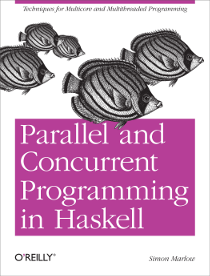
\includegraphics[scale=0.45]{parcur.png} 
\columnbreak

Wunderbares Buch zum Thema von Simon Marlow.\pause\bigskip

Gratis im Internet verfügbar, inklusive Beispielcode.
\end{multicols}

\end{frame}

\subsection{Motivation}

%----------------------------------------------------------------------------------------

\begin{frame}[fragile]

\begin{center}
\Large
\textbf{Motivation}
\end{center}

\end{frame}

%----------------------------------------------------------------------------------------

\begin{frame}[fragile]

\begin{center}
\huge
\emph{Free Lunch is over!}\bigskip

\normalsize
Herb Sutter (2005)
\end{center}
\pause
Die Hardware unserer Computer wird seit mehreren Jahren schon schneller breiter (\emph{mehr} Kerne) als tiefer (\emph{schnellere} Kerne).\pause\smallskip

Um technischen Fortschritt voll auszunutzen ist es also essentiell, gute Werkzeuge für einfache und effiziente Parallelisierung bereit zu stellen.
\end{frame}

%----------------------------------------------------------------------------------------

\subsection{Definitionen}

\begin{frame}[fragile]

\begin{center}
\Large
\textbf{Definitionen}
\end{center}

\end{frame}

\section{Parallelism}

%----------------------------------------------------------------------------------------

\begin{frame}

\begin{center}
\Large
\textbf{Parallelism}\normalsize\bigskip

\begin{itemize}
\item Die \texttt{Eval}-Monade und Strategies
\item Die \texttt{Par}-Monade
\item Die \texttt{RePa}-Bibliothek
\item GPU-Programming mit \texttt{Accelerate}
\end{itemize}
\end{center}

\end{frame}

%----------------------------------------------------------------------------------------

\subsection{Die Eval-Monade und Strategies}

\begin{frame}[fragile]

\begin{center}
\Large
\textbf{Parallelism}\normalsize\bigskip
\begin{itemize}
\item $\circ$ Die \texttt{Eval}-Monade und Strategies
\item Die \texttt{Par}-Monade
\item Die \texttt{RePa}-Bibliothek
\item GPU-Programming mit \texttt{Accelerate}
\end{itemize}
\end{center}

\end{frame}

%----------------------------------------------------------------------------------------

\begin{frame}[fragile]

Das Modul \texttt{Control.Parallel.Strategies} (aus dem Paket \texttt{parallel}) stellt uns
die \texttt{Eval}-Monade und einige Funktionen vom Typ \emph{Strategy} zur Verfügung, \dots\pause

\mint{haskell}|    type Strategy a = a -> Eval a|
\pause

\dots insbesondere die Strategies \texttt{rpar} und \texttt{rseq}. Dazu gleich mehr.\pause\bigskip

Desweiteren stellt es die Operation \texttt{runEval}, die die monadischen 
Berechnungen ausführt und das Ergebnis zurück gibt, bereit.

\mint{haskell}|    runEval :: Eval a -> a|
\pause
\bigskip

Wohlgemerkt: \texttt{runEval} ist \emph{pur!}

Wir müssen nicht gleichzeitig auch in der \texttt{IO}-Monade sein.

\end{frame}

%----------------------------------------------------------------------------------------

\subsection{Die Par-Monade}

\begin{frame}[fragile]

\begin{center}
\Large
\textbf{Parallelism}\normalsize\bigskip
\begin{itemize}
\item Die \texttt{Eval}-Monade und Strategies
\item $\circ$ Die \texttt{Par}-Monade
\item Die \texttt{RePa}-Bibliothek
\item GPU-Programming mit \texttt{Accelerate}
\end{itemize}
\end{center}

\end{frame}

%----------------------------------------------------------------------------------------

\subsection{Die RePa-Bibliothek}

\begin{frame}[fragile]

\begin{center}
\Large
\textbf{Parallelism}\normalsize\bigskip
\begin{itemize}
\item Die \texttt{Eval}-Monade und Strategies
\item Die \texttt{Par}-Monade
\item $\circ$ Die \texttt{RePa}-Bibliothek
\item GPU-Programming mit \texttt{Accelerate}
\end{itemize}
\end{center}

\end{frame}

%----------------------------------------------------------------------------------------

\subsection{Accelerate}

\begin{frame}[fragile]

\begin{center}
\Large
\textbf{Parallelism}\normalsize\bigskip
\begin{itemize}
\item Die \texttt{Eval}-Monade und Strategies
\item Die \texttt{Par}-Monade
\item Die \texttt{RePa}-Bibliothek
\item $\circ$ GPU-Programming mit \texttt{Accelerate}
\end{itemize}
\end{center}

\end{frame}

%----------------------------------------------------------------------------------------

\end{document}